\section{Theory}

\subsection{Control flow graphs}
\begin{figure}[h]
    \begin{subfigure}{0.5\textwidth}
        \centering
        \tikzset{%
  % Specifications for style of nodes:
         base/.style = {rectangle, rounded corners, draw = black, minimum width=2.5cm, minimum height=1cm, fill=orange!15, font=\ttfamily},
}

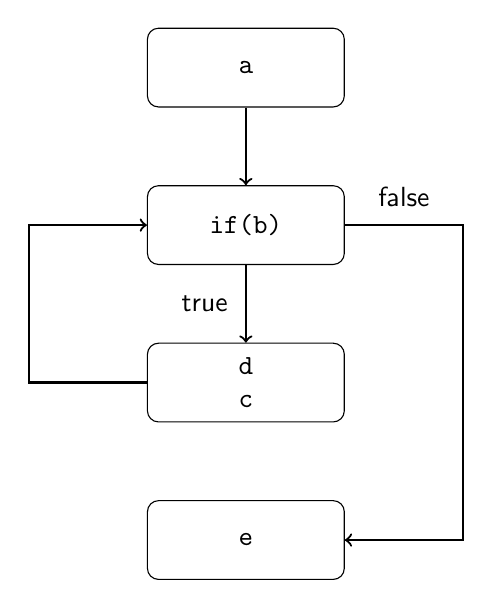
\begin{tikzpicture}[node distance=2cm, every node/.style={fill=white, font=\sffamily}, align=center]
    % Draw nodes
    \node (start)       [base]                        {a};
    \node (if)          [base, below of = start]      {if(b)};
    \node (incr)        [base, below of = if]       {d\\c};
    \node (end)         [base, below of = incr]       {e};

    % Draw arrows
    \draw[->,thick]           (start) -- (if);
    \draw[->,thick]            (if) -- node[left = 0.1cm, midway] {true} (incr);

    \draw[->,thick]            (incr.west) -- ++(-1.5,0) -- ++(0,2) -- ++(1.5,0) (if);
    \draw[->,thick]         (if.east) -- node[above = 0.1cm,midway] {false} ++(1.5,0) -- ++(0,-4) -- ++(-1.5,0)     (end);


\end{tikzpicture}

        \caption{Control flow graph for for loop}
        \label{fig:cfg_for}
    \end{subfigure}%
    ~
    \begin{subfigure}{0.5\textwidth}
        \centering
        \tikzset{%
  % Specifications for style of nodes:
         base/.style = {rectangle, rounded corners, draw = black, minimum width=2.5cm, minimum height=1cm, fill=orange!15, font=\ttfamily},
}

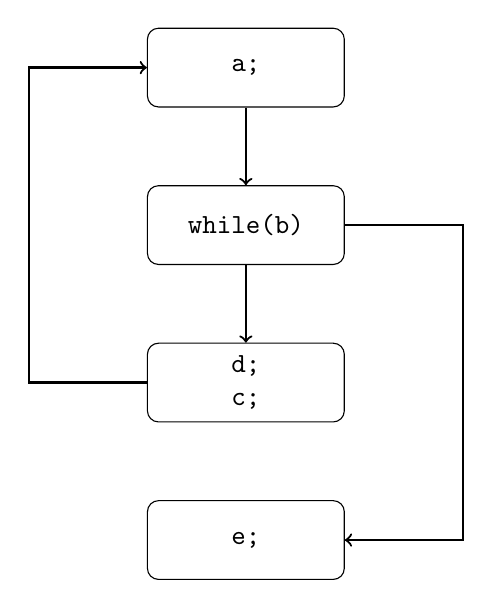
\begin{tikzpicture}[node distance=2cm, every node/.style={fill=white, font=\sffamily}, align=center]
    % Draw nodes
    \node (start)       [base]                        {a;};
    \node (while)       [base, below of = start]      {while(b)};
    \node (code)        [base, below of = while]      {d;\\c;};
    \node (end)         [base, below of = code]       {e;};

    % Draw arrows
    \draw[->,thick]           (start) -- (while);
    \draw[->,thick]           (while) -- (code);

    \draw[->,thick]       (code.west) -- ++(-1.5,0) -- ++(0,4) -- ++(1.5,0)         (while);
    \draw[->,thick]       (while.east) -- ++(1.5,0) -- ++(0,-4) -- ++(-1.5,0)     (end);


\end{tikzpicture}

        \caption{Control flow graph for while loop}
        \label{fig:cfg_while}
    \end{subfigure}
    \par\bigskip\medskip
    \centering
    \begin{subfigure}{0.5\textwidth}
        \centering
        
\tikzset{%
  % Specifications for style of nodes:
         base/.style = {rectangle, rounded corners, draw = black, minimum width=2.5cm, minimum height=1cm, fill=orange!15, font=\ttfamily},
}

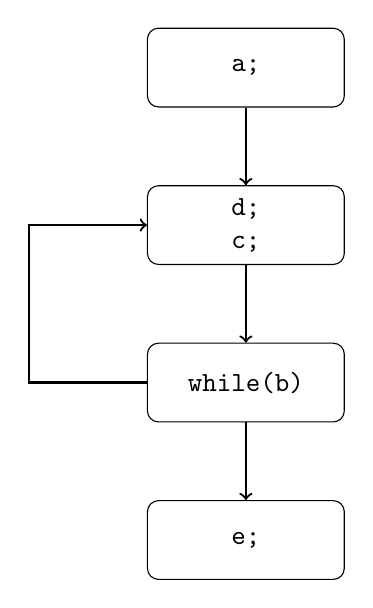
\begin{tikzpicture}[node distance=2cm, every node/.style={fill=white, font=\sffamily}, align=center]
    % Draw nodes
    \node (start)       [base]                        {a;};
    \node (do)          [base, below of = start]      {d; \\ c;};
    \node (while)       [base, below of = do]         {while(b)};
    \node (end)         [base, below of = while]      {e;};

    % Draw arrows
    \draw[->,thick]           (start) -- (do);
    \draw[->,thick]           (do) -- (while);
    \draw[->,thick]           (while) -- (end);

    \draw[->,thick]           (while.west) -- ++(-1.5,0) -- ++(0,2) -- ++(1.5,0) (do);
\end{tikzpicture}

        \caption{Control flow graph for do-while loop}
        \label{fig:cfg_do_while}
    \end{subfigure}
\end{figure}


\newpage
\subsection{Program fragment}
\subsubsection{Control flow graph of program fragment}
\begin{figure}[h]
    \centering
    \tikzset{%
  % Specifications for style of nodes:
         base/.style =  { rectangle, rounded corners, draw = black, minimum width=2.5cm, minimum height=1cm, font=\ttfamily },
         node/.style =  { base, fill=orange!15 },
         begin/.style = { base, fill=blue!30 },
         end/.style =   { base, fill=red!30 },
}

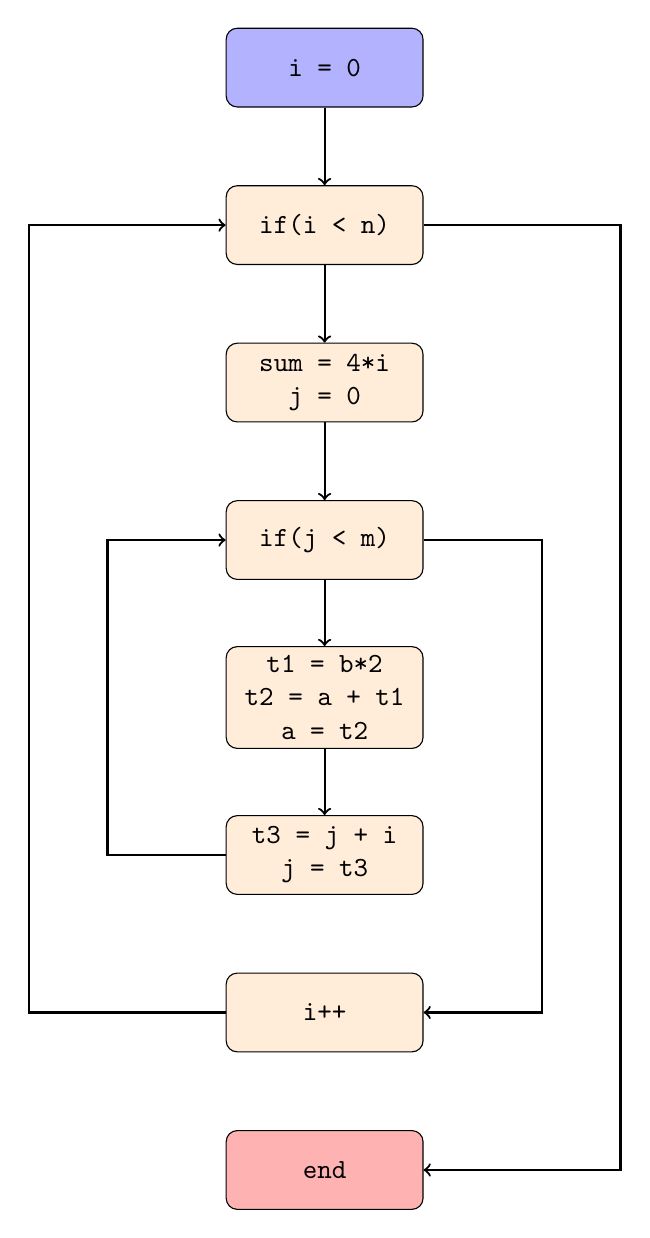
\begin{tikzpicture}[node distance=2cm, every node/.style={fill=white, font=\sffamily}, align=center]
    % Draw nodes
    \node (start)       [begin]                        {i = 0};
    \node (if_1)        [node, below of = start]       {if(i < n)};
    \node (block)       [node, below of = if_1]        {sum = 4*i \\ j = 0};
    \node (if_2)        [node, below of = block]       {if(j < m)};
    \node (block_2)     [node, below of = if_2]        {t1 = b*2 \\ t2 = a + t1 \\ a = t2};
    \node (block_3)     [node, below of = block_2]     {t3 = j + i \\ j = t3};
    \node (block_4)     [node, below of = block_3]     {i++};
    \node (end)         [end, below of = block_4]      {end};

    % Draw arrows
    \draw[->,thick]           (start) -- (if_1);
    \draw[->,thick]           (if_1) -- (block);
    \draw[->,thick]           (block) -- (if_2);
    \draw[->,thick]           (if_2) -- (block_2);
    \draw[->,thick]           (block_2) -- (block_3);

    \draw[->,thick]           (block_3.west) -- ++(-1.5,0) -- ++(0,4) -- ++(1.5,0) (if_2);
    \draw[->,thick]           (if_2.east) -- ++(1.5,0) -- ++(0,-6) -- ++(-1.5,0) (block_3);
    \draw[->,thick]           (block_4.west) -- ++(-2.5,0) -- ++(0,10) -- ++(2.5,0) (if_1);
    \draw[->,thick]           (if_1.east) -- ++(2.5,0) -- ++(0,-12) -- ++(-2.5,0) (end);
\end{tikzpicture}

    \caption{Control flow graph for program fragment}
    \label{fig:cfg_program}
\end{figure}

\subsubsection{Dominator equations}\label{sec:dom_eq}
\begin{subequations}
    \begin{align}
        D(1) &= \{1\}\\
        D(2) &= D(1) \cup \{2\} = \{1,2\}\\
        D(3) &= D(2) \cup \{3\} = \{1,2,3\}\\
        D(4) &= D(3) \cup \{4\} = \{1,2,3,4\}\\
        D(5) &= D(4) \cup \{5\} = \{1,2,3,4,5\}\\
        D(6) &= D(4) \cup \{6\} = \{1,2,3,4,6\}\\
        D(7) &= D(2) \cup \{7\} = \{1,2,7\}
    \end{align}
\end{subequations}

\subsubsection{Dominator tree}
\begin{figure}[h]
    \centering
    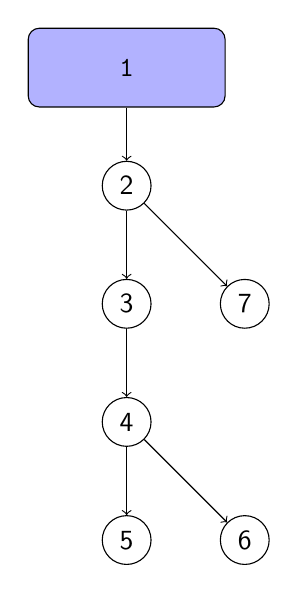
\begin{tikzpicture}[node distance=1.5cm, every node/.style={circle, draw = black, fill=white, font=\sffamily}, align=center]
    % Draw nodes
    \node (start)   [begin]             {1};
    \node (2)       [below of = start]  {2};
    \node (3)       [below of = 2]      {3};
    \node (4)       [below of = 3]      {4};
    \node (5)       [below of = 4]      {5};
    \node (6)       [right of = 5]      {6};
    \node (7)       [right of = 3]      {7};

    % Draw arrows
    \draw[->] (start) -- (2);
    \draw[->] (2) -- (3);
    \draw[->] (3) -- (4);
    \draw[->] (4) -- (5);
    \draw[->] (2) -- (7);
    \draw[->] (4) -- (6);
\end{tikzpicture}

    \caption{Dominator tree from equations in \cref{sec:dom_eq}}
\end{figure}

\section{Code}
See attached code. Run bash run\_all.sh to compile compiler, compile vsl-programs and run with predetermined input.
